\section{Organigramm}

In diesem Kapitel wird die Organisationsstruktur des kompletten Projektes erläutert. Dabei stellte das fünfte Semester die Konzeptionierungsphase und das sechste Semester die Umsetzungsphase dar. Dementsprechend wurden in beiden Phasen individuelle Arbeitsgruppen gebildet.

\subsection{5. Semester}
Während des fünften Semesters befand sich das Projekt in der Konzeptionierungsphase. Für diese wurde das Projektteam in vier Teams eingeteilt. Dementsprechend haben alle Teammitglieder an der Umsetzung der Aufgaben teilgenommen, die Verantwortung für einzelne Aufgaben wurde jedoch auf diese vier Teams verteilt. Im Folgenden werden diese Teams und deren dazugehörige Aufgabe dargestellt:

\begin{description}
\item[Kommunikation mit PulseShift\\]\hfill \\
- Schnittstelle zu PulseShift\\
- Organisieren und Leiten von Meetings mit PulseShift\\
- Abgleich der Anforderungen von PulseShift mit der Ausführung


\item[Ideengenerierung und Sammlung]\hfill \\
- Generierung von Ideen z.B. durch eine Design Thinking Session\\
- Sammeln von Ideen aus dem Team\\
- Festhalten und Ausarbeitung von Ansätzen

\item[Projektmanagementtools]\hfill \\
	- Auswahl von relevanten Projektmanagementtools und Diagrammen\\
	- Erstellung von Diagrammen

\item[Projektmanagement]\hfill \\
	\textbf{Scrum Master:}\\
	\phantom{hue}- Terminieren und Organisieren von Team-Meetings\\
	\phantom{hue}- Aufstellen einer Agenda\\
	\phantom{hue}- Trello Board verwalten\\\\
	\textbf{Qualitätsmanagement}\\
	\phantom{hue}- Protokollerstellung\\
	\phantom{hue}- Sicherstellung der Qualität von Arbeitsausführung und -ergebnissen\\
	\phantom{hue}- Kommunikation mit Herr Holey
\end{description}

In \vref{organigramm_semester5} sind die zuvor beschriebenen Teams und deren dazugehörigen Mitglieder grafisch abgebildet.

\begin{figure}[h]
\centering
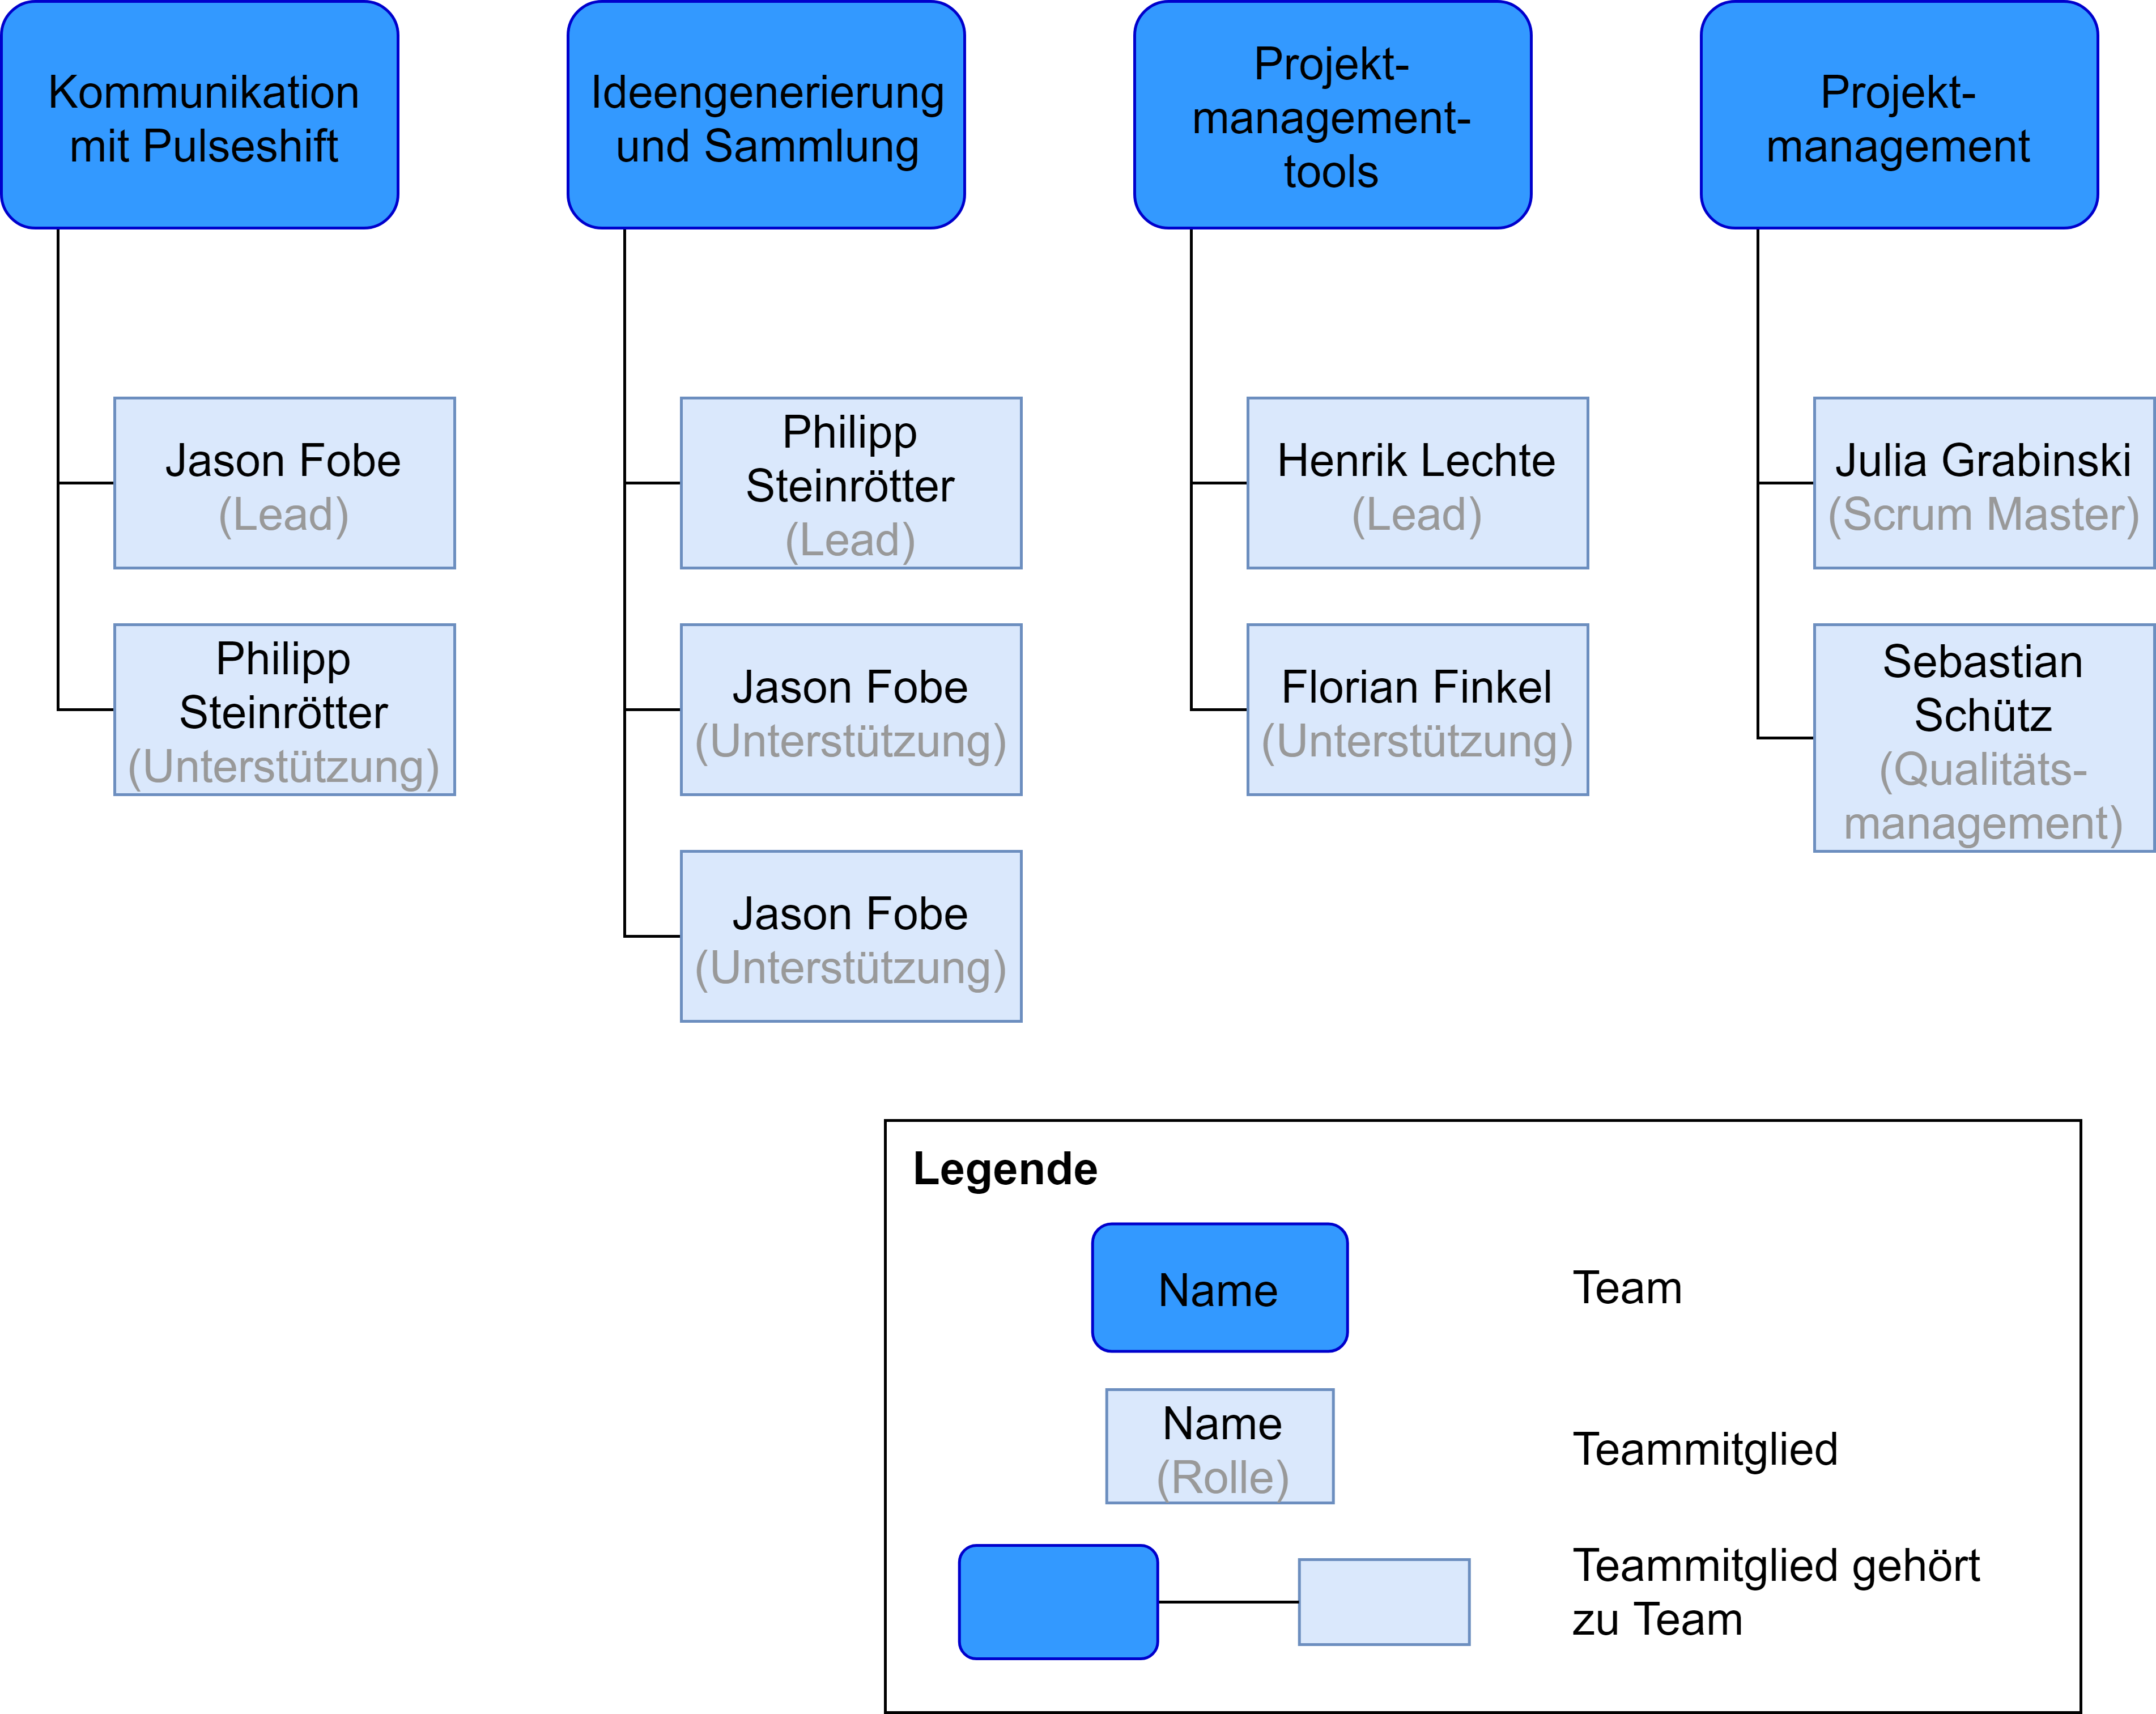
\includegraphics[width=12cm]{images/organigramm_semester5}
\caption{Bildliche Darstellung der Organisation während der \\ Konzeptiomsphase im 5. Semester\protect}
\label{organigramm_semester5}
\end{figure}

\subsection{6. Semester}

Im anschließenden sechsten Semesters wurde auf Basis der Konzeptionierungsphase die Umsetzungsphase initiiert und vollendet. Dabei wurden sowohl die im fünften Semester etablierten Teams beibehalten und deren Aufgaben fortgesetzt als auch neue Arbeitsgruppen gebildet, die für die Umsetzung einzelner Konzeptionen verantwortlich waren. Nachfolgend werden diese neu entstandene Arbeitsgruppen und deren entsprechenden Pflichten dargelegt:

\begin{description}
\item[Lunchapp]\hfill \\
- Entwickelt Single-Purpose-Webapp\\
- Informationen über Essenspläne werden angezeigt\\
- Push-Notifications weißen auf mögliche Umfragen hin


\item[Newsfeed App Research]\hfill \\
- Untersucht bereits vorhandene Apps im Markt\\
- Überprüft ob PulseShift diese Apps für Umfragen nutzen kann

\item[Captive Portal]\hfill \\
- Untersucht Hardwarelösungen mit Captive Portal Funktionalität\\
- Realisiert die Captive Portal Funktionalität mit genau einer Hardwarelösung\\
- Ermöglichen Weiterleitung der Teilnehmer zur Umfrage

\item[Dokumentation \& Projektmanagement]\hfill \\
- Vorgabe für Dokumentation \& Protokollierung der Umsetzung\\
- Qualitätssicherung der einzelnen Arbeitsgruppen\\
- Erstellung einer Gesamtdokumentation
\end{description}

In \vref{organigramm_semester5} ist der zuvor erläuterte Aufbau der Organisation visualisiert.

\begin{figure}[h]
\centering
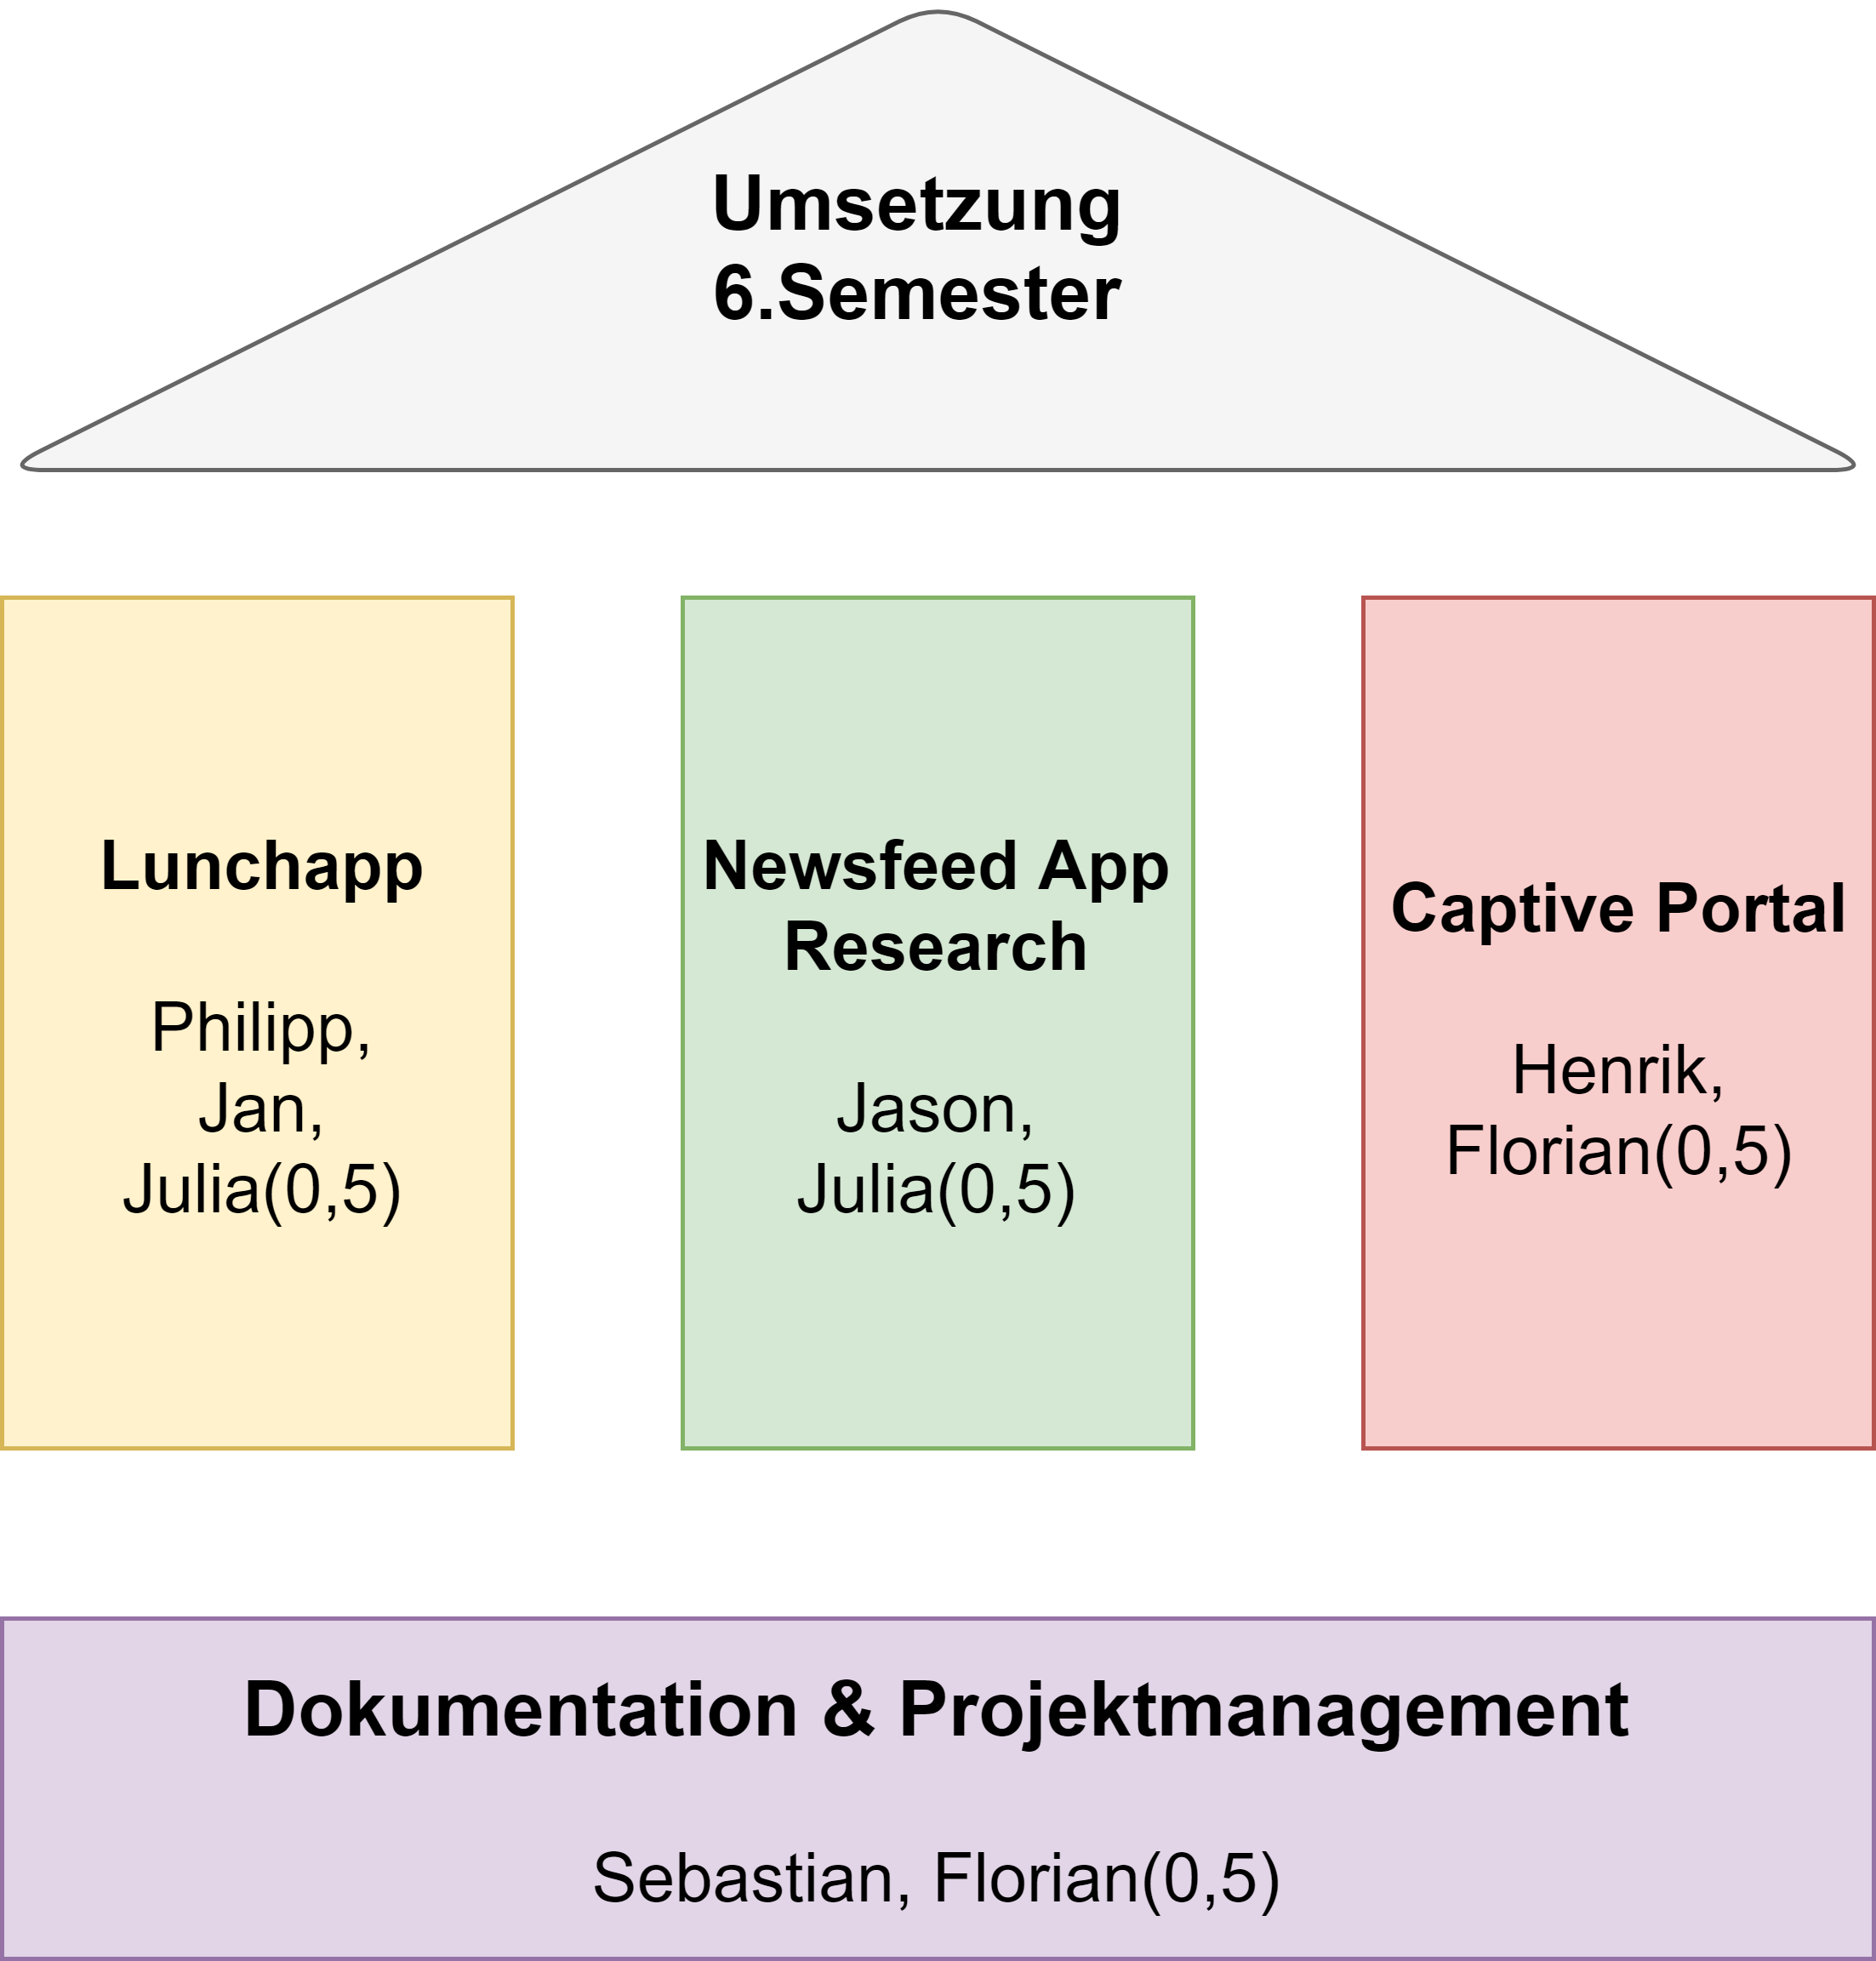
\includegraphics[width=9cm]{images/organigramm_semester6}
\caption{Bildliche Darstellung der Organisation während der Umsetzungsphase im 6. Semester\protect}
\label{organigramm_semester6}
\end{figure}